\section*{\centering Reproducibility Summary}

% \textit{Template and style guide to \href{https://paperswithcode.com/rc2020}{ML Reproducibility Challenge 2020}. The following section of Reproducibility Summary is \textbf{mandatory}. This summary \textbf{must fit} in the first page, no exception will be allowed. When submitting your report in OpenReview, copy the entire summary and paste it in the abstract input field, where the sections must be separated with a blank line.

\subsection*{Scope of Reproducibility}
% State the main claim(s) of the original paper you are trying to reproduce (typically the main claim(s) of the paper).
% This is meant to place the work in context and to tell a reader the objective of the reproduction.
The original work by  \cite{xiang2020interpretable} claimed (1) that complex-valued DNNs effectively increase the difficulty of inferring inputs for the adversary attacks compared to the baseline. 
In addition, \cite{xiang2020interpretable} stated that the (2) proposed privacy-protecting complex-valued DNN effectively preserves the accuracy when compared to the baseline.

\subsection*{Methodology}

% Briefly describe what you did and which resources you used. For example, did you use the author's code? Did you re-implement parts of the pipeline? You can also use this space to list the hardware used and the total budget (e.g. GPU hours) for the experiments. 

Since the original paper's code was not published, all of the codebase was written independently from scratch, based solemnly on how it was described in the paper. We mostly used a Nvidia's \textit{RTX 2060 Super} as the GPU and a \textit{AMD Ryzen 3600x} as the CPU.  The runtime of each model was highly dependant on the architecture used. The runtimes for each model can be found in Table \ref{runtime-table}.
\subsection*{Results}
% Start with your overall conclusion --- where did your results reproduce the original paper, and where did your results differ? Be specific and use precise language, e.g. "we reproduced the accuracy to within 1\% of reported value, which supports the paper's conclusion that it outperforms the baselines". Getting the same number is in most cases infeasible, so you'll need to use your judgment to decide if your results support the original claim of the paper.
In contrast to the first claim, we have discovered that for most of the architectures, reconstruction errors for the attacks are quite low, which means that in our models the first claim is not supported. We also found that for most of the models, the classification error is somewhat higher than those provided in the paper. However, these indeed relate to the original work and partially support the second claim of the authors.


\subsection*{What was easy}
Authors of the original paper utilized famous architectures for some of architectures' parts, such as ResNet and LeNet, that were well explained and defined in the literature. In addition, authors, provided formulas on the modified rotation-invariant Complex DNN modules (ReLU, max pooling etc.), implementation of which was relatively straightforward. The paper was based on the openly available datasets. 

\subsection*{What was difficult}
The paper did not provide  any information on the architecture of the critic for the WGAN, along with the architecture of the angle discriminator utilized in inversion attack 1. It also does not  provide any information about crucial hyperparameters, such as the k value used for k-anonimity.

% Describe which parts of your reproduction study were difficult or took much more time than you expected. Perhaps the data was not available, and you couldn't verify some experiments, or the author's code was broken and had to be debugged first. Or, perhaps some experiments just take too much time/resources to run and you couldn't verify them. The purpose of this section is to indicate to the reader which parts of the original paper are either difficult to re-use, or require a significant amount of work and resources to verify.

\subsection*{Communication with original authors}

% Briefly describe how much contact you had with the original authors (if any).
We did not contact the original authors of the publication.

% \textit{\textbf{The following section formatting is \textbf{optional}, you can also define sections as you deem fit.
% \\
% Focus on what future researchers or practitioners would find useful for reproducing or building upon the paper you choose.}}

%%%%%%%%%%%%%%%%%%%%%%%%%%%%%%%%%%%%%%%%%%%%%%%%%%%%%%%%%%%%%%%%%%%
\newpage
\section{Introduction}
% [A few sentences placing the work in high-level context. Limit it to a few paragraphs at most; your report is on reproducing a piece of work, you don't have to motivate that work.]

Deep Neural Networks (DNNs) can process a massive data volume but require great computing power to process this data. Therefore it is an interesting option for small devices like smartphones or IoT devices to use a cloud operator for these computationally expensive tasks. Although this is an efficient way to process data, the cloud operator is susceptible to privacy threats. A potential attacker could reconstruct or infer private properties of the data. Possible solutions are subject of current research.

\cite{xiang2020interpretable} proposed a possible solution using encryption and complex-valued neural networks to address this problem. They showed that their approach increases the difficulty of inferring inputs or properties from intermediate layer features. Our paper aims at reproducing their findings.

 \cite{xiang2020interpretable} extended the standard DNN by encrypting the intermediate layer features using complex-valued DNNs (\cite{DBLP:journals/corr/TrabelsiBSSSMRB17}). The local device encodes the original input into intermediate features. Those features are encrypted and sent to a processing unit, a complex-valued neural net located in the cloud. It does the computationally expensive operations while not being able to infer properties of its input. The result is sent back to the local device and decrypted.
 
 Ideally, the local device is able to decrypt the encoded data using the secret key. However, an adversary shouldn't be able to decrypt the features without the key.  \cite{xiang2020interpretable} achieved this by rotating intermediate layer features into the complex plane using a random angle. The angle acts as a key and can be used to reverse the rotation. The processing unit consists of rotation-invariant operations only. Thus, the local device can reverse the rotation after receiving the results from the processing unit. To make it hard to deduce the angle, a generative adversarial network is trained to alter the intermediate features to introduce obfuscation whilst keeping important information.
 

% \begin{figure}[H]
%     \centering
%     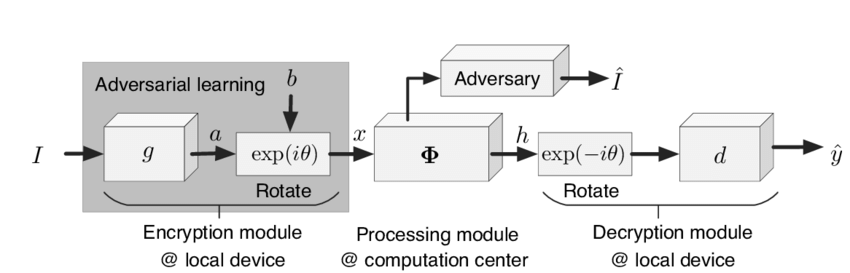
\includegraphics[width=0.7\linewidth]{\detokenize{../openreview/images/complex-network.png}}
%     \captionof{figure}{Structure of the complex-valued neural network}
%     \label{complex-network}
% \end{figure}

%%%%%%%%%%%%%%%%%%%%%%%%%%%%%%%%%%%%%%%%%%%%%%%%%%%%%%%%%%%%%%%%%%%

\section{Scope of reproducibility}
\label{sec:claims}
% Introduce the specific setting or problem addressed in this work and list the main claims from the original paper. Think of this as writing out the main contributions of the original paper. Each claim should be relatively concise; some papers may not clearly list their claims, and one must formulate them in terms of the presented experiments. (For those familiar, these claims are roughly the scientific hypotheses evaluated in the original work.)

% A claim should be something that can be supported or rejected by your data. An example is, "Finetunipre-trainedned BERT on dataset X will have higher accuracy than an LSTM trained with GloVe embeddings."
% This is concise, and is something that can be supported by experiments.
% An example of a claim that is too vague, which can't be supported by experiments, is "Contextual embedding models have shown strong performance on a number of tasks. We will run experiments evaluating two types of contextual embedding models on datasets X, Y, and Z."

% This section roughly tells a reader what to expect in the rest of the report. Clearly itemize the claims you are testing:
% \begin{itemize}
%     \item Claim 1
%     \item Claim 2
%     \item Claim 3
% \end{itemize}

% Each experiment in Section~\ref{sec:results} will support (at least) one of these claims, so a reader of your report should be able to separately understand the \emph{claims} and the \emph{evidence} that supports them.

The main problem \cite{xiang2020interpretable} addresses is the danger of adversary attackers being able to recover original inputs or hidden properties of the input. 
\cite{xiang2020interpretable} claim their complex-valued model to be robust against these kinds of adversary attacks and show this by attacking their model with various inversion and inference attacks. Here, they claim that attacking their complex-valued DNNs acquires greater reconstruction loss than when they attack the original DNNs, meaning they are more resistant to adversary attacks. Furthermore, even though the input is encoded, they claim that their complex-valued DNNs have almost the same utility performance (classification error rates) as the original DNNs. 

In this paper, we test the following concrete claims:
\begin{enumerate}
    \item \cite{xiang2020interpretable} proposed complex-valued DNNs effectively boost the difficulty of inferring inputs for the adversary compared to the baseline. \label{claim1}
    \item \cite{xiang2020interpretable} proposed their privacy-preserving complex-valued DNN largely preserves the accuracy when compared to the baseline. \label{claim2}
\end{enumerate}

%\jdcomment{To organizers: I asked my students to connect the main claims and the experiments that supported them. For example, in this list above they could have "Claim 1, which is supported by Experiment 1 in Figure 1." The benefit was that this caused the students to think about what their experiments were showing (as opposed to blindly rerunning each experiment and not considering how it fit into the overall story), but honestly, it seemed hard for the students to understand what I was asking for.}

%%%%%%%%%%%%%%%%%%%%%%%%%%%%%%%%%%%%%%%%%%%%%%%%%%%%%%%%%%%%%%%%%%%

\section{Methodology}
% Explain your approach - did you use the author's code, or did you aim to re-implement the approach from the description in the paper? Summarize the resources (code, documentation, GPUs) that you used.

The paper from \cite{xiang2020interpretable} was replicated \footnote{Our implementation can be found at our GitHub (\cite{github-gana-fact-ai})} by solely using the methods described in their paper, since there was no implementation available online. Our approach involved implementing the models used by \cite{xiang2020interpretable}, which included the ResNet-$\alpha,\beta$-20/32/44/56/110 (\cite{DBLP:journals/corr/HeZRS15}), the LeNet (\cite{lecun1998gradient}), the VGG-16 (\cite{simonyan2015deep}) and the AlexNet (\cite{NIPS2012_c399862d}). Most of these papers had implementations available online, which were adjusted slightly to be able to process complex-valued intermediate layer features. Furthermore, these DNNs had to be disassembled to create the complex-valued DNN structure proposed by \cite{xiang2020interpretable} that consists of an encoder, processing module and decoder.

The encoder is in principle the same as the first few layers of the used DNN, but at the end of the encoder a complex rotation is applied (Eq. \ref{eq_rotate_forward}).

\begin{equation}
    x = \exp(i\theta)[a+bi]
    \label{eq_rotate_forward}
\end{equation}

The value a represents the regular input that is put through the encoder. The value b is the fooling counterpart that can be seen as a different input that is also put through the encoder. Theta is picked to be random angle, which will act as the secret key we mentioned earlier.

The resulting features are then fed to the processing unit. The processing unit consists of the middle layers of the used DNN. The processing unit has to deal with complex features, which means adjustments had to be made to the regular functions that the DNN uses. We used the proposed functions in \cite{DBLP:journals/corr/TrabelsiBSSSMRB17} to achieve this. Furthermore it is important that the processing unit does not change the rotation of the features, because otherwise if we try to rotate it back with our randomly picked angle we will get random results. Therefore we also had to make the used functions rotation invariant. Methods for achieving this were described in \cite{xiang2020interpretable}.

Finally the features are put through the decoder, which consists of the final layers of the used DNN. The decoder first rotates the features back with the randomly picked angle (Eq. \ref{eq_decoder}) and then feeds the result to the final layers.

\begin{equation}
    \hat{y} = d(R[h \exp(-i\theta)])
    \label{eq_decoder}
\end{equation}

The value h represents the output of the processing unit and the value $\hat{y}$ is the prediction that the decoder d made.

\cite{xiang2020interpretable} also uses a Wasserstein Generative Adversarial Network which was proposed by \cite{pmlr-v70-arjovsky17a} and is part of the encoder. This WGAN consists of a generator and a critic that use complex rotations to teach the network to generate synthesized features to hide the original ones. Since no implementation with a WGAN that works with complex-valued features was available online, this WGAN encoder had to be completely remade.

Lastly, for the adversary attacks, \cite{xiang2020interpretable} attacked the model with inversion and inference attacks. For the inversion attacks, we adopted the U-net model proposed by \cite{U-net}, which had similar variants online that had to be hardly modified to fit their implementation. For the inference attack, a model had to be implemented that functions as a classifier to predict hidden properties of the input.

\subsection{Model descriptions}
\subsubsection{Complex-valued DNNs}
In \cite{xiang2020interpretable} approach, the DNN is split into two local parts that are used to encode and decode the data (encoder and decoder, respectively) and a middle part that performs all of the heavy data processing (processing module). 

In the original work, two ResNet implementations were described: ResNet-$\alpha$ and ResNet-$\beta$. In ResNet-$\alpha$ the input is transformed until the first 16x16 feature map, from where the output is sent to the encoder. After the encoding, the processing module transforms the data until the first 8x8 feature map. From that point on, all following layers constitute to the decoder. The difference in ResNet-$\beta$ is that the decoder was composed by the last residual block and the layers following it. 

% need to rewrite the following part since it's almost the exact words from the paper
% -> 
For describing the other classical DNNs, we only specify the encoder and the decoder, where all the remaining layers contribute to the processing unit. For the LeNet model, the encoder consisted of the first convolutional layer and the WGAN, whereas the decoder contained only the softmax layer. In the VGG-16 all layers before the last 56x56 feature map constituted the encoder. Here, the decoder consisted of fully-connected layers and the softmax layer. For the AlexNet, the first three convolutional layers' output was fed into the encoder, where the decoder contained fully-connected layers and the softmax layer.

\subsubsection{WGAN}
To introduce obfuscation and make it hard for the adversary to reconstruct the original features, a WGAN is utilized. A WGAN is a variant of a generative adversarial network known to be more resistant against hyperparameters or mode collapse compared to the original approach. The WGANs encoder is used to introduce obfuscation to the features. The critic is only used to train the generator, and its objective is to distinguish rotated features from those without rotation. The generator of the WGAN shares the same network as the encoder we described earlier. This means that one part of the network (the encoder/generator) is trained with two different purposes; One is for classification and the other is for the WGAN. To train the generator, the encoded and rotated (Eq. \ref{eq_rotate_forward}) features it produced are passed to the critic, which is trying to retrieve the original features by rotating the given features back. 
\begin{equation}
    a' = \Re[x \exp(-i\theta']
    \label{eq_rotate_back}
\end{equation}
The critic creates k-1 fake samples and rotates them by k-1 randomly sampled angles $\theta'$ (Eq. \ref{eq_rotate_back}), where $\theta'\neq\theta$. The critic then discriminates whether these rotated features are close to the original complex-valued features.

From  \cite{xiang2020interpretable}, it was unclear whether the generator is only a part of the encoder or whether the WGAN trains all encoder layers. Because no architecture was given for the generator, we decided to train all the encoder layers with the WGAN loss and not introduce a stand-alone generator after the encoder.

% The original WGAN uses weight clipping for the Discriminator in order to enforce the Lipshitz-constraint. However, we found that this constraint was too harsh and that all the weights of the critic converged to the clipping value after a few iterations. Because of this behavior, it was impossible to train the WGAN appropriately. We found that this is a common problem with WGANs. \cite{DBLP:journals/corr/GulrajaniAADC17} suggested a solution to this problem using a gradient penalty. Instead of using weight clipping to enforce the Lipshitz-constraint, they added a penalty to the loss function if the gradient norm was not close to 1. Using this approach solved our problem and yielded reasonable gradients.

The original WGAN uses weight clipping for the critic network. However we found that all the weights converged to the clipping values rather quickly. Because of this we cannot train the WGAN appropriately. To fix this issue we used a gradient penalty which was introduced in \cite{DBLP:journals/corr/GulrajaniAADC17}.

\subsubsection{Adversary models}
% Include a description of each model or algorithm used. Be sure to list the type of model, the number of parameters, and other relevant info (e.g. if it's pretrained). 

\textbf{Inversion attacks}\\
The objective of the inversion attack was to reconstruct the input images from the encoded intermediate features. \cite{xiang2020interpretable} implemented two inversion attacks: in inversion attack 1 a new discriminator ($D'$) is first trained to predict the most probable features ($a^*$) by learning the most likely angle at which the intermediate layer features are rotated (Eq. \ref{theta}). The most probable features (Eq. \ref{astar}) are then used to help train a decoder model that tries to reconstruct the original images (Eq. \ref{ihat}). In inversion attack 2 the angle prediction discriminator is not included and the attacker only trains a decoder that tries to reconstruct the original images from the given intermediate layer features. 

\begin{align}
    \hat{\theta} &= \max_{\theta}D'(\Re[x\exp(-i\hat{\theta}) \label{theta} \\
    a^* &= \Re[x\exp(-i\hat{\theta}] \label{astar} \\
    \hat{I} &= \text{dec}(a^*) \label{ihat}
\end{align}

The structure of the reconstruction model for both inversion attacks was based on a modified U-Net (\cite{U-net}) described in the original work. U-Net is a neural network architecture widely used for image segmentation. It is based on an Autoencoder architecture decorated by skip connections. The skip connections help to reconstruct the exact low-level attributes such as the location of edges. Intermediate layer features from the encoder are scaled up to the original input size and then fed into the U-Net, aiming to reconstruct the original image. 

% In case when the input of an adversary, i.e, feature tensor $x$, had dimensions smaller than that of the original image, it was up-sampled to the size of the 


\textbf{Inference attacks}\\
During inference attacks a classifier is trained on either similar raw images (inference 1), rotated features $a^*$ (inference 2) or fully reconstructed images $\hat{I}$ (inference 3). Furthermore, a model is trained using k-nearest neighbors (k-NNs), where the attacker compares $a^*$ against features of each training example to find similarities in the training set. We did not implement the inference attacks, because the results of the inversion attacks showed that the privacy protection was not working properly. Instead of implementing the inference attacks, which would yield similar poor results, we decided to investigate further into why the privacy protection was not working.

% Due to time constraints we were not able to implement the inference attacks.

\subsection{Datasets}
% For each dataset include 1) relevant statistics such as the number of examples and label distributions, 2) details of train / dev / test splits, 3) an explanation of any preprocessing done, and 4) a link to download the data (if available).

\cite{xiang2020interpretable} used CIFAR-10/100 (\cite{cifar10}, \cite{cifar100}) to train the ResNets and LeNet, CUB-200 (\cite{WelinderEtal2010}) to train VGG-16 and CelebA (\cite{CelebA}) for AlexNet. Since we did not implement VGG-16 and AlexNet, we only used the CIFAR-10/100 datasets using the train/test split described in Table \ref{dataset}. Each split was halved to create two smaller datasets used for training/testing either the privacymodel or the adversary attacker. Before training, all datasets were normalized. 

\begin{table*}[t]
    \centering
    \setlength{\abovecaptionskip}{5pt}
    \caption{Relevant statistics for the used datasets}
    \begin{tabular}{l||l|l|l}
    \hline
    \textbf{Dataset} & \textbf{Labels} & \textbf{Number of examples} & \textbf{Split (train/dev/test)} \\
    \hline 
    CIFAR-10 & 10 & 60.000 & 50.000 / 0 / 10.000 \\
    CIFAR-100 & 100 & 600.000 & 500.000 / 0 / 100.000 \\
    % CUB-200 & 200 & 6.033 & ? \\
    % CelebA & 10177 & 202.599 & ? \\
    \end{tabular}
    \label{dataset}
\end{table*}

\subsection{Hyperparameters}
% Describe how the hyperparameter values were set. If there was a hyperparameter search done, be sure to include the range of hyperparameters searched over, the method used to search (e.g., manual search, random search, Bayesian optimization, etc.), and the best hyperparameters found. Include the number of total experiments (e.g. hyperparameter trials). You can also include all results from that search (not just the best-found results).

Unfortunately, none of the standard hyperparameters such as learning rate, optimizer, weight decay, etc. were mentioned in the paper. Therefore we had to adapt and choose them ourselves. For the WGAN, we used the hyperparameters given in the original implementation by \cite{pmlr-v70-arjovsky17a}.  We implemented weight clipping and gradient penalty. For the first one, we used RMSprop with a learning rate of $5e^{-5}$ for both the generator and the critic. Weights were clipped between $-0.01$ and $0.01$ for the Critic's weights. 

As this learning rate was too low for the classification task, we used a different optimizer. Adam was used with a learning rate of $5e^{-4}$. For the gradient penalty approach, we set lambda to $10$ and used Adam with a learning rate of $5e^{-4}$. We did not do an intensive hyperparameter search to optimise these parameters.

Finally, another hyperparameter specific to this paper is called k. k represents the number of times the discriminator decides on an input per iteration. The discriminator always has to calculate a real score based on the real features a, so there are k-1 fake inputs that determine the fake score. This hyperparameter is also never defined in the paper. We set the k value on 8, and we have not been able to test other options, unfortunately. 

We trained our adversary networks with the Adam optimizer and a learning rate of $5e^{-4}$. For training the U-net we used the Mean Squared Error loss and for training the angle predictor network we used the Absolute Mean loss.


\subsection{Experimental setup and code}
% Include a description of how the experiments were set up that's clear enough a reader could replicate the setup. 
% Include a description of the specific measure used to evaluate the experiments (e.g. accuracy, precision@K, BLEU score, etc.). 
% Provide a link to your code.

Since PyTorch currently does not fully support complex-valued tensors, we chose to split up the 'real' part and the 'imaginary part' into two tensors, where we have created new complex functions to process these two tensors correctly.

We introduced complex and, most-importantly, rotation-invariant ReLU, BatchNorm, and MaxPool layers according to the original work's formulae.
In addition, we have also discovered that for Complex Linear Layers, the bias term should not be involved in matrix computations, even though it was only mentioned for the case Complex Convolutional Layers in the original paper. 

The architecture of processing unit is designed so that after the the features $x$ from encoder are passed through processing unit, we could express the output as a complex rotation of outputs of processing unit, i.e $\Phi(x)$, specifically it means:

\begin{equation}
    \Phi(e^{i \theta}x) = e^{i \theta} \Phi (x)
    \label{eq4}
\end{equation}

To keep the equation \label{eq4} true for the Convolutional Linear Layers $\Phi(e^{i \theta} x )$ and $e^{i \theta} \Phi(x)$ should be equal to each other, meaning that for:
\begin{equation}
    \Phi(e^{i \theta}x) = w  \cdot (e^{i \theta}x) + b  
    \label{eq2}
\end{equation}

\begin{equation}
    e^{i \theta} \Phi (x) = e^{i \theta} (w \cdot x + b)
    \label{eq3}
\end{equation}

Given any $\theta$, we see that the equality would hold only if b = 0, which would mean that no bias term would be needed. Thi is exactly the objective of rotation invariance for our network as it was mentioned in the publication.

In the original work, the Critic's architecture was not described, so some assumptions regarding its architecture were made. We found that one linear layer is not sufficient. Thus, we added a convolution, a ResNet block and another convolution.
Since the LeNet network looks very different from the ResNet networks we decided to change to the critic architecture to look more like the generator of LeNet.

In the paper, they describe how the decoder of the AlexNet only consists of a softmax layer. This is not possible, because they train the network on the attributes of CelebA and since multiple attributes per image are used, introduction of a sigmoid function is essential. The output of the last layer in the decoder is a sigmoid and the binary cross-entropy loss is applied in order to estimate how well it assigns attributes to each image.

The paper implements inversion and inference attacks to test whether it is preserving the privacy. For inversion attack 1 it uses a network to determine the angle that was most likely used for rotation. We decided to implement this network by creating a network that is identical to the critic that we used for that specific network.

The U-Net architecture used in the inversion attacks is constructed using 6 convolutional layers per block, instead of the standard 2 convolutional layers per block. Furthermore, the U-net architecture consisted of 4 down and 4 upsampling blocks. Each downsampling block reduced the features' dimensions by 2, while the up-sampling ones doubled the aforementioned dimensions. Thus, input and output image widths and heights were preserved.

We found that the inversion attacks were reconstructing the images very well when we used them on our trained networks. Adding a convolution layer without a ReLU activation function to our generator increased the overall reconstruction loss, effectively making our network preserve the privacy better. This was further improved by randomly swapping a and b in our generator, which lead to a significant increase in the reconstruction loss.

From all the networks that were used in \cite{xiang2020interpretable} we implemented LeNet and the ResNet-32/44/56/110-$\alpha, \beta$ architectures. We did not implement the other architectures, because the ResNet and LeNet architectures showed that the privacy protection was not working as described. We decided to continue our investigation into ResNet and LeNet, instead of implementing more networks which would face the same problems as ResNet and LeNet.

% Unfortunately we were not able to get AlexNet and VGG-16 to properly work as they both returned NaN after a certain duration of training. We could not find the cause of this issue and because of the time constraint we had to give up on these networks. The networks can still be found in the github on different branches than the main branch, but no good results can be produced with them.

\subsection{Computational requirements}
% Include a description of the hardware used, such as the GPU or CPU the experiments were run on. 
% For each model, include a measure of the average runtime (e.g. average time to predict labels for a given validation set with a particular batch size).
% For each experiment, include the total computational requirements (e.g. the total GPU hours spent).
% (Note: you'll likely have to record this as you run your experiments, so it's better to think about it ahead of time). Generally, consider the perspective of a reader who wants to use the approach described in the paper --- list what they would find useful.

We mostly used a RTX 2060 super for the GPU and a ryzen 3600x for the CPU. The runtime of each model was highly dependant on the architecture used. The runtimes for each model can be found in Table \ref{runtime-table}.

% \begin{table*}[t]
%     \centering
%     \scalebox{0.9}{
%     \begin{tabular}{l||l}
%     \hline
%     \textbf{Model} & \textbf{Average Runtime} \\
%     \hline
%     LeNet & 48 m \\
%     % ResNet-20-$a$ & 2h 34m \\
%     % ResNet-20-$b$ & 2h 28m \\
%     ResNet-32-$a$ & 2h 29m \\
%     ResNet-32-$b$ & 2h 41m \\
%     ResNet-44-$a$ & 3h 15m \\
%     ResNet-44-$b$ & 3h 08m \\
%     ResNet-56-$a$ & 3h 34m \\
%     ResNet-56-$b$ & 3h 23m \\
%     ResNet-110-$a$ & 3h 20m \\
%     ResNet-110-$b$ & 3h 12m \\
%     \end{tabular}
%     }
%     \caption{Average runtime for each model}
%     \label{runtime-table}
% \end{table*}

\begin{table}[!htb]
    \begin{minipage}{.5\linewidth}
    \setlength{\abovecaptionskip}{5pt}
    \caption{Average runtime for each model}
    \centering
  
    \begin{tabular}{l||l}
    \hline
    \textbf{Model} & \textbf{Average Runtime} \\
    \hline
    LeNet & 48 m \\
    % ResNet-20-$a$ & 2h 34m \\
    % ResNet-20-$b$ & 2h 28m \\
    ResNet-32-$a$ & 2h 29m \\
    ResNet-32-$b$ & 2h 41m \\
    ResNet-44-$a$ & 3h 15m \\
    ResNet-44-$b$ & 3h 08m \\
    ResNet-56-$a$ & 3h 34m \\
    ResNet-56-$b$ & 3h 23m \\
    ResNet-110-$a$ & 3h 20m \\
    ResNet-110-$b$ & 3h 12m \\
    \end{tabular}
    
    \label{runtime-table}
        
    \end{minipage}%
    \begin{minipage}{.5\linewidth}
    
    \centering
    \setlength{\abovecaptionskip}{5pt}
    \caption{Inversion attack 1 and 2 results}
    \scalebox{0.9}{
    \begin{tabular}{l|c|c|c|c}
    \hline
    \multicolumn{1}{c|}{} & \multicolumn{2}{|c|}{Inversion Attack 1} &  \multicolumn{2}{|c}{Inversion Attack 2} \\
    \hline
    \textbf{Model} & \textbf{Paper} & \textbf{Reproduced} & \textbf{Paper} & \textbf{Reproduced}\\
    \hline
    LeNet & 0.2405 & 0.1499 & 0.1027 & 0.1244 \\
    ResNet-32-$\alpha$ & 0.2569 & 0.0277 & 0.2412 & 0.0464 \\
    ResNet-32-$\beta$ & 0.2515 & 0.0292 & 0.2425 & 0.0323 \\
    ResNet-44-$\alpha$ & 0.2746 & 0.0256 & 0.2419 & 0.0293 \\
    ResNet-44-$\beta$ & 0.2511 & 0.0190 & 0.2397 & 0.0383 \\
    ResNet-56-$\alpha$ & 0.2804 & 0.1031 & 0.2377 & 0.0399 \\
    ResNet-56-$\beta$ & 0.2585 & 0.0242 & 0.2358 & 0.0483 \\
    ResNet-110-$\alpha$ & 0.3081 & 0.0292 & 0.2495 & 0.0447 \\
    ResNet-110-$\beta$ & 0.2582 & 0.0207 & 0.2414 & 0.0321 \\
    
    \end{tabular}
    }
    
    \label{inversion-table}
    \end{minipage} 
\end{table}

\section{Results}
\label{sec:results}
% Start with a high-level overview of your results. Do your results support the main claims of the original paper? Keep this section as factual and precise as possible, reserve your judgement and discussion points for the next "Discussion" section. 

\subsection{Results reproducing original paper}
% For each experiment, say 1) which claim in Section~\ref{sec:claims} it supports, and 2) if it successfully reproduced the associated experiment in the original paper. 
% For example, an experiment training and evaluating a model on a dataset may support a claim that that model outperforms some baseline.
% Logically group related results into sections. 
In these sections we show the results produced by our network and relate them to the claims introduced in section 2.

\subsubsection{Increased difficulty of inferring inputs}
In this section we show the results that relate to the first claim (\ref{claim1}) based on what our initial implementation of our networks produced.
Table \ref{inversion-table} shows the reconstruction errors of multiple different networks with the old implementation when attacked with inversion attack 1 and 2. The table shows that the reconstruction errors of our networks are much lower than the reconstruction errors of the paper's networks. We can therefore say that the first claim is not supported by these networks.
The reconstructed images that were created by inversion attack 1 on the ResNet-32-$\alpha$ network can be seen in Figure \ref{resnet32}. The reconstructed images look very similar to the original images, further proving that the first claim is not supported.

% \begin{table*}[t]
%     \centering
%     \scalebox{0.7}{
%     \begin{tabular}{l|c|c|c|c}
%     \hline
%     \multicolumn{1}{c|}{} & \multicolumn{2}{|c|}{Inversion Attack 1} &  \multicolumn{2}{|c}{Inversion Attack 2} \\
%     \hline
%     \textbf{Model} & \textbf{Paper} & \textbf{Reproduced} & \textbf{Paper} & \textbf{Reproduced}\\
%     \hline
%     LeNet & 0.2405 & 0.1509 & 0.1027 & 0.1244 \\
%     ResNet-32-$\alpha$ & 0.2569 & 0.0277 & 0.2412 & 0.0464 \\
%     ResNet-32-$\beta$ & 0.2515 & 0.0292 & 0.2425 & 0.0323 \\
%     ResNet-44-$\alpha$ & 0.2746 & 0.0256 & 0.2419 & 0.0293 \\
%     ResNet-44-$\beta$ & 0.2511 & 0.0190 & 0.2397 & 0.0383 \\
%     ResNet-56-$\alpha$ & 0.2804 & 0.1031 & 0.2377 & 0.0399 \\
%     ResNet-56-$\beta$ & 0.2585 & 0.0242 & 0.2358 & 0.0483 \\
%     ResNet-110-$\alpha$ & 0.3081 & 0.0292 & 0.2495 & 0.0447 \\
%     ResNet-110-$\beta$ & 0.2582 & 0.0207 & 0.2414 & 0.0321 \\
%     \end{tabular}
%     }
%     \caption{Inversion attack 1 and 2 results}
%     \label{inversion-table}
% \end{table*}

% \begin{figure}[!h]
%     \centering
%     \includegraphics[width=0.24\textwidth]{../openreview/original images.png}
%     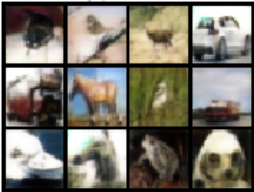
\includegraphics[width=0.24\textwidth]{../openreview/reconstructed images.png}
%     \caption{Original images on the left, reconstructed images on the right}
%     \label{fig:images_resnet_32_a}
% \end{figure}

\begin{figure}[!tbp]
    \centering
    \begin{subfigure}{.5\textwidth}
      \centering
      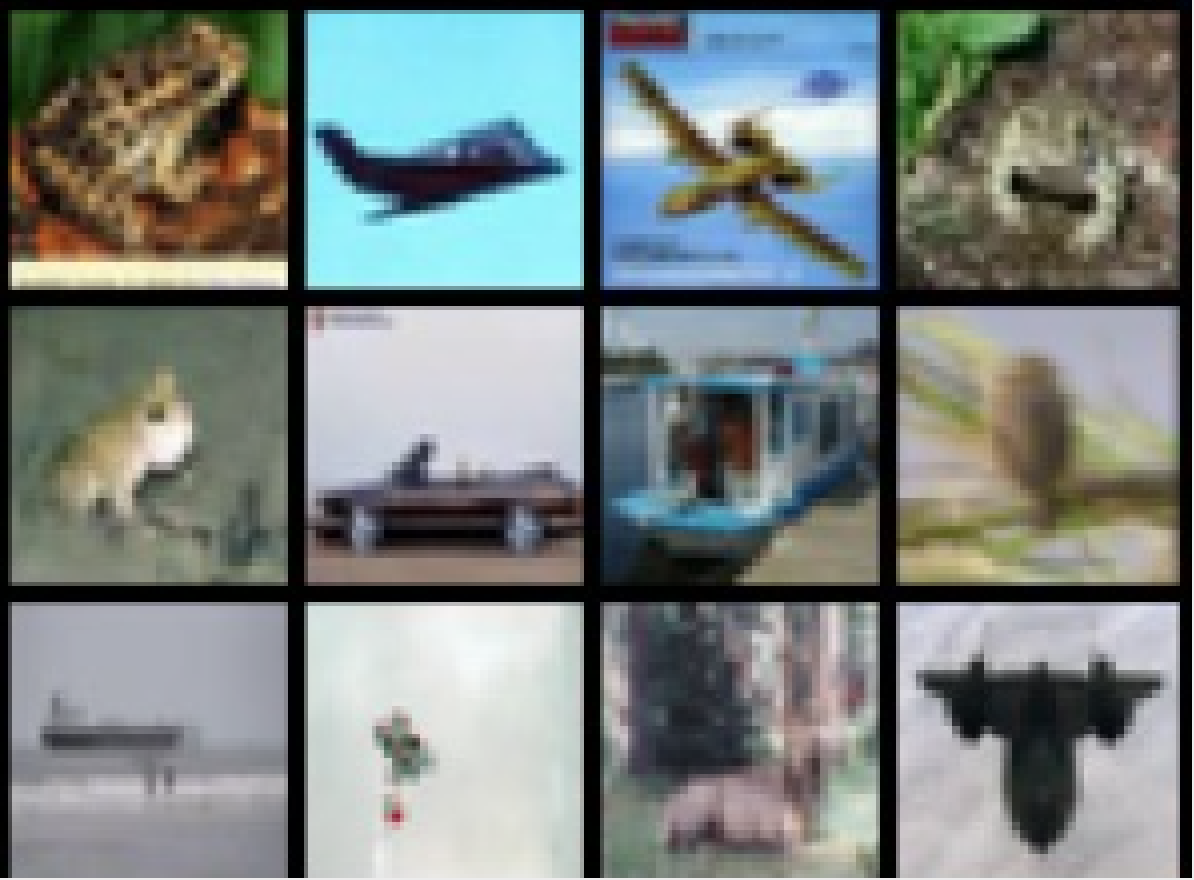
\includegraphics[width=0.45\textwidth]{../openreview/lenet_original.png}
        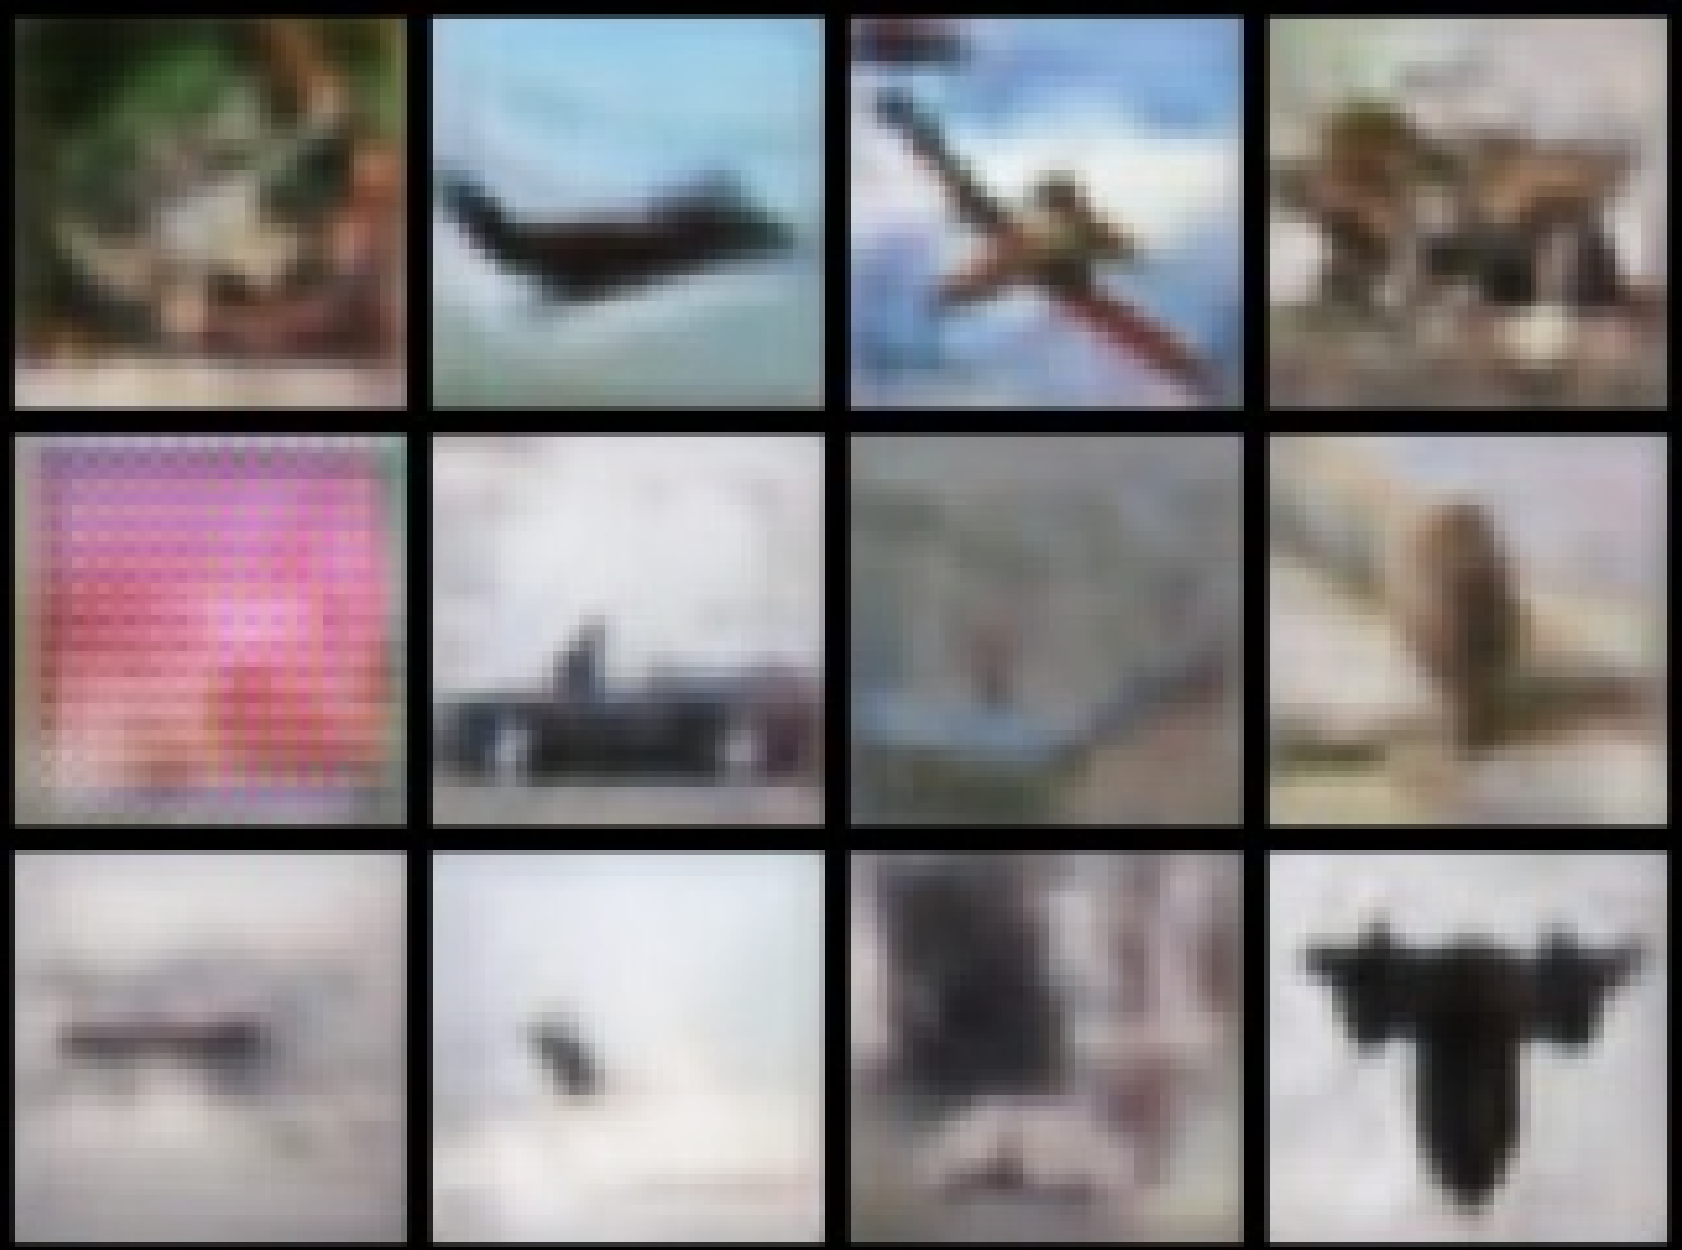
\includegraphics[width=0.45\textwidth]{../openreview/lenet_reconstruct.png}
        \captionsetup{labelformat=empty}
        \caption{LeNet-5 architecture}
        \label{lenet5}
    \end{subfigure}%
    \begin{subfigure}{.5\textwidth}
        \captionsetup{labelformat=empty}
        \includegraphics[width=0.45\textwidth]{../openreview/original images.png}
        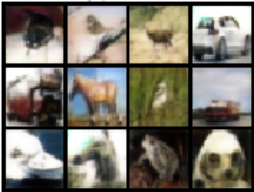
\includegraphics[width=0.45\textwidth]{../openreview/reconstructed images.png}
        \caption{ResNet-32-$\alpha$ architecture}
        \label{resnet32}
    \end{subfigure}
    \captionsetup{justification=centering}
    \caption{Image reconstruction after inversion attack 1. Original images on the left, \\ reconstructed images on the right of each atchitecture}
    \label{fig:reconstruction}
\end{figure}

% \begin{figure}[!tbp]
%   \centering
%   \begin{minipage}[b]{0.45\textwidth}
%     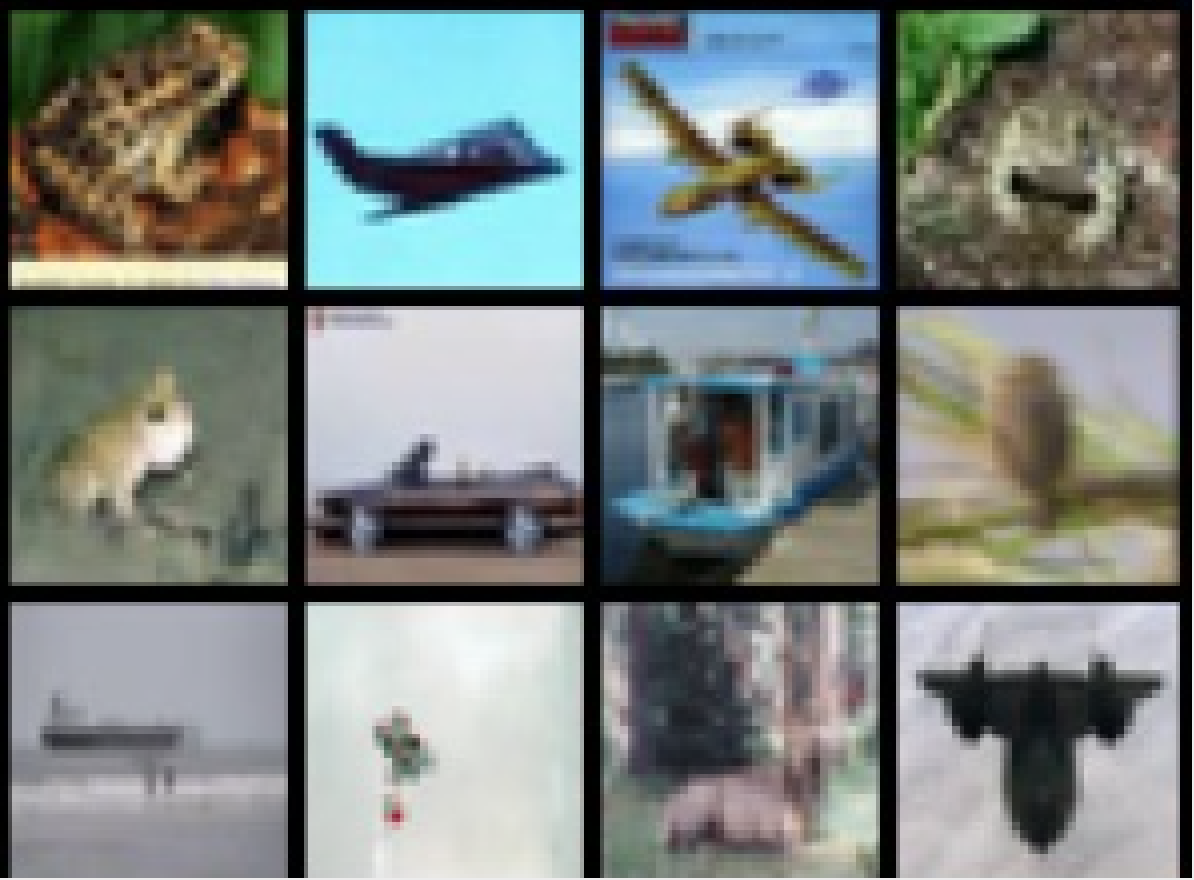
\includegraphics[width=0.45\textwidth]{../openreview/lenet_original.png}
%     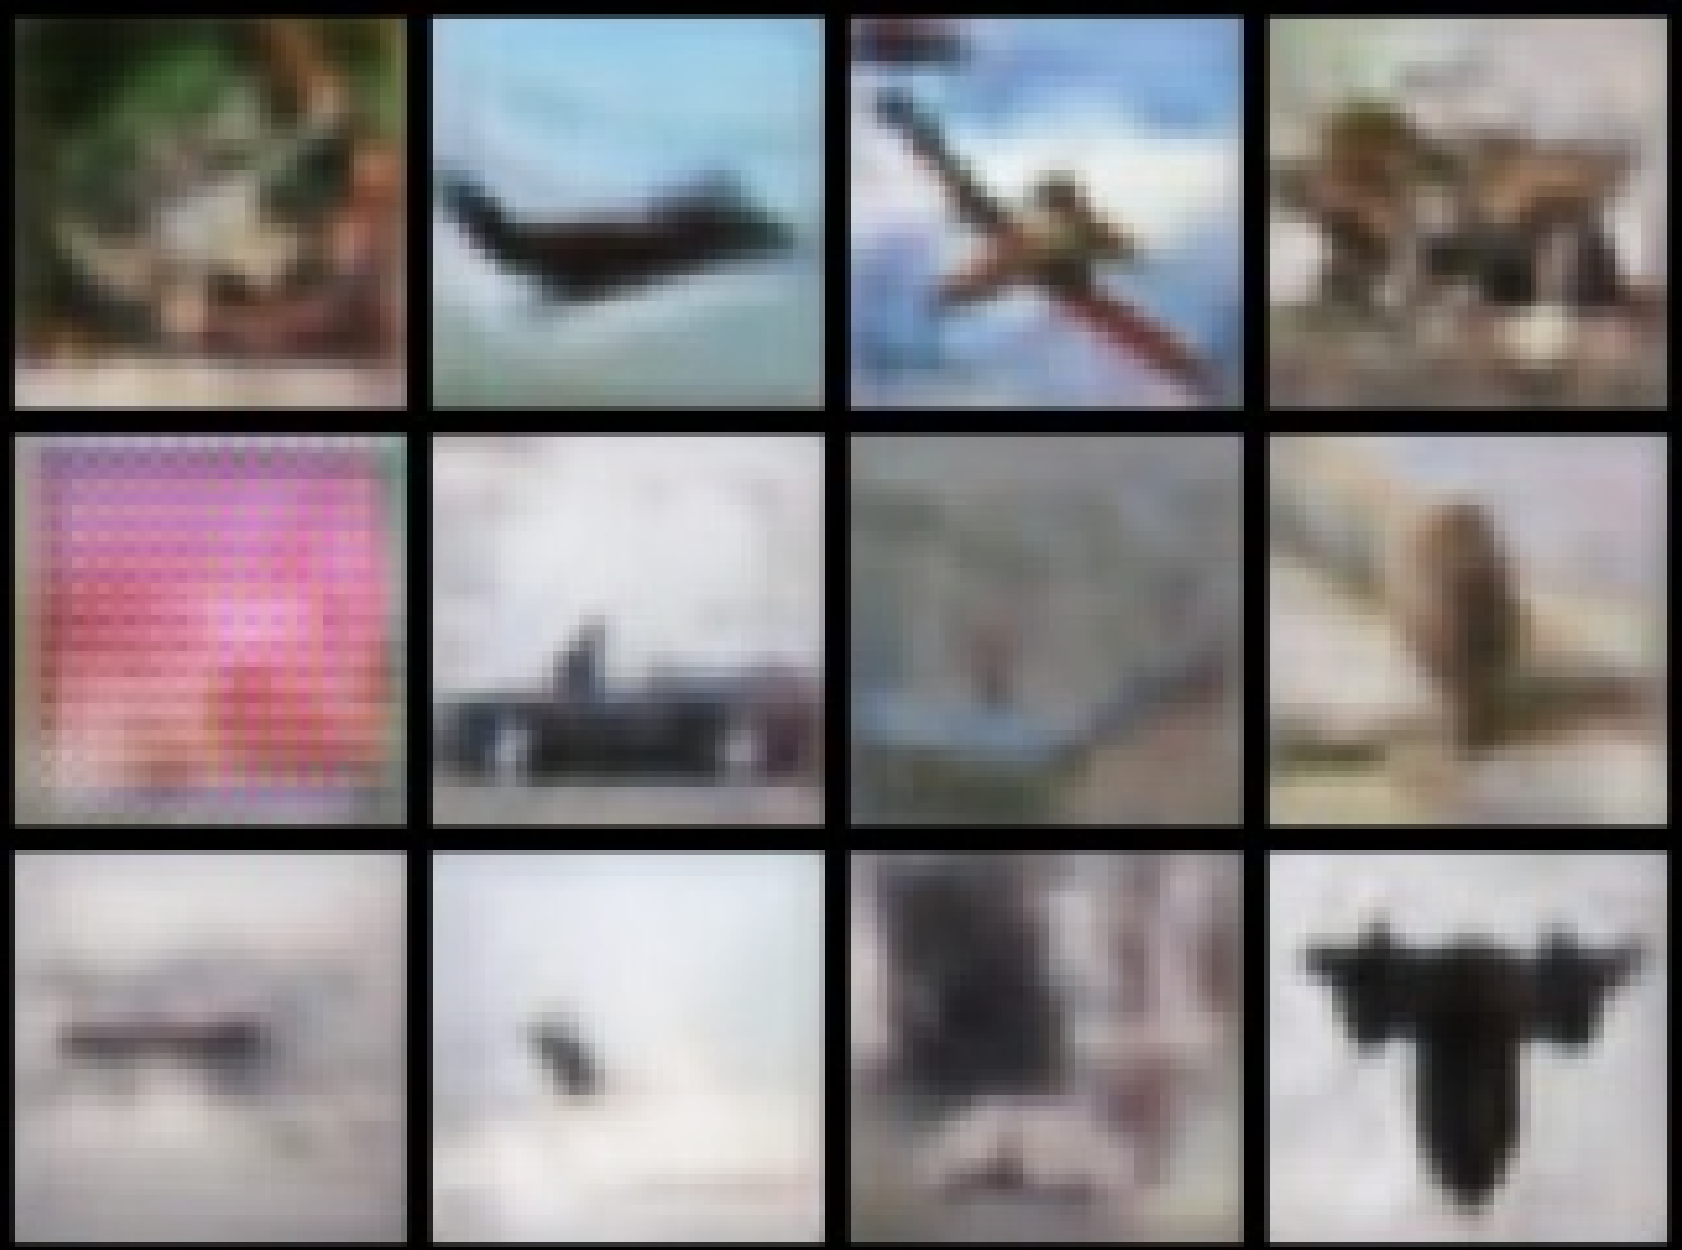
\includegraphics[width=0.45\textwidth]{../openreview/lenet_reconstruct.png}
%     \captionsetup{labelformat=empty}
%     \caption{LeNet-5 architecture}
%     \label{lenet5}
%   \end{minipage}
%   \hfill
%   \begin{minipage}[b]{0.45\textwidth}
%     \captionsetup{labelformat=empty}
%     \includegraphics[width=0.45\textwidth]{../openreview/original images.png}
%     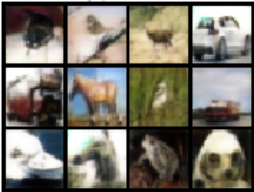
\includegraphics[width=0.45\textwidth]{../openreview/reconstructed images.png}
%     \caption{ResNet-32-$\alpha$ architecture}
%     \label{resnet32}
%   \end{minipage}
%   \caption{Image reconstruction after inversion attack 1. Original images on the left, reconstructed images on the right of each atchitecture}
%   \label{fig:reconstruction}
% \end{figure}


In Table \ref{inversion-table} we can see the results of attacking our new implementation network with inversion attack 1 and 2. Here we see that the results look a lot more similar and we can therefore say that the first claim is supported under our new implementation. This claim is further supported by Figure \ref{fig:reconstruction} where the reconstructed images can be seen of the new implementation network.

\subsubsection{Preservation of accuracy}
In this section we show the results that relate to the second claim (\ref{claim2}). 
Table \ref{accuracy-table} shows the classification errors of the old implementation of our networks. The table shows that our network's classification errors are quite a bit higher than the paper's classification errors. However our network's classification errors are still quite low, which is why the results partially support the second claim.
In table \ref{accuracy-table} we can see the classification errors of the new implementation of our networks. We see that the classification error is quite similar to the old implementation and therefore also partially supports the second claim.

% \begin{table}
% 	\begin{minipage}{0.5\linewidth}
% 		\caption{Student Database}
% 		\label{table:student}
% 		\centering
% 		\begin{tabular}{lrr}
% 			\toprule
% 			Student          & h/week & Grade \\
% 			\midrule
% 			Ada Lovelace     & 2      & A \\
% 			Linus Thorvalds  & 8      & A \\
% 			Bruce Willis     & 12     & F \\
% 			Richard Stallman & 10     & B \\
% 			Grace Hopper     & 12     & A \\
% 			Alan Turing      & 8      & C \\
% 			Bill Gates       & 6      & D \\
% 			Steve Jobs       & 4      & E \\
% 			\bottomrule
% 		\end{tabular}
% 	\end{minipage}\hfill
% 	\begin{minipage}{0.45\linewidth}
% 		\centering
% 		\includegraphics[width=40mm]{\detokenize{../openreview/original images.png}}
% 		\captionof{figure}{2-D scatterplot of the Student Database}
% 		\label{ }
% 	\end{minipage}
% \end{table}

\begin{table}
	\begin{minipage}{0.5\linewidth}
		\centering
		\captionsetup{justification=centering}
		\setlength{\abovecaptionskip}{5pt}
		\caption{Classification Errors of the paper's results (left) and the reproduced results (right)}
        % \scalebox{0.75}{
        \begin{tabular}{l|c|c}
        \hline
        \multicolumn{1}{c|}{} & \multicolumn{2}{|c}{Classification Error} \\
        \hline
        \textbf{Model} & \textbf{Paper} & \textbf{Reproduced} \\
        \hline
        LeNet & 17.95 & 59.62 \\
        ResNet-32-$\alpha$ & 10.48 & 19.53 \\
        ResNet-32-$\beta$ & 11.12 & 25.00 \\
        ResNet-44-$\alpha$ & 11.08 & 26.09 \\
        ResNet-44-$\beta$ & 10.51 & 26.48 \\
        ResNet-56-$\alpha$ & 11.53 & 25.78 \\
        ResNet-56-$\beta$ & 11.28 & 28.91 \\
        ResNet-110-$\alpha$ & 11.97 & 24.22 \\
        ResNet-110-$\beta$ & 11.85 & 28.17 \\
        \end{tabular}
        % }
        
        \label{accuracy-table}
	\end{minipage}\hfill
	\begin{minipage}{0.45\linewidth}
    	\centering
    	\setlength{\abovecaptionskip}{5pt}
        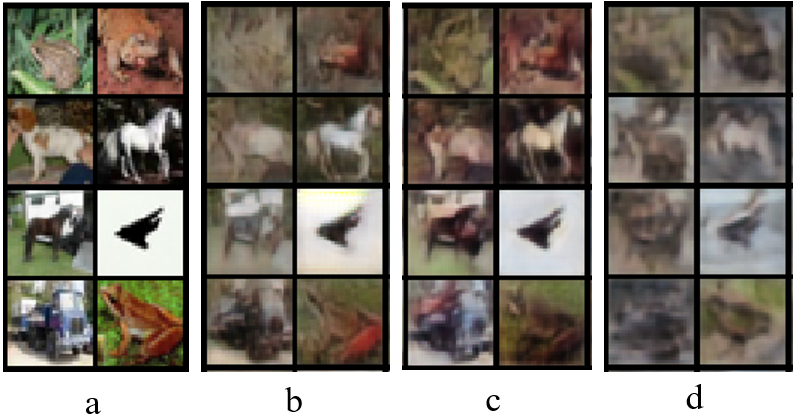
\includegraphics[width=0.9\textwidth]{../openreview/images/image_reconstructions.PNG}
        \captionof{figure}{Image reconstructions, trained on Cifar10 and ResNet-22-$\alpha$. a) Original images. b) Model without ReLU at the end of the generator. c) Model with ReLU at the end of the generator. d) Model trained while randomly swapping a and b; The WGAN was not trained, however, the adversary is not able to reconstruct the inputs. Also, the accuracy of the classifier didn't change using this approach.}
        \label{fig:kanonymity}
	\end{minipage}
\end{table}

\begin{figure}
    \centering
    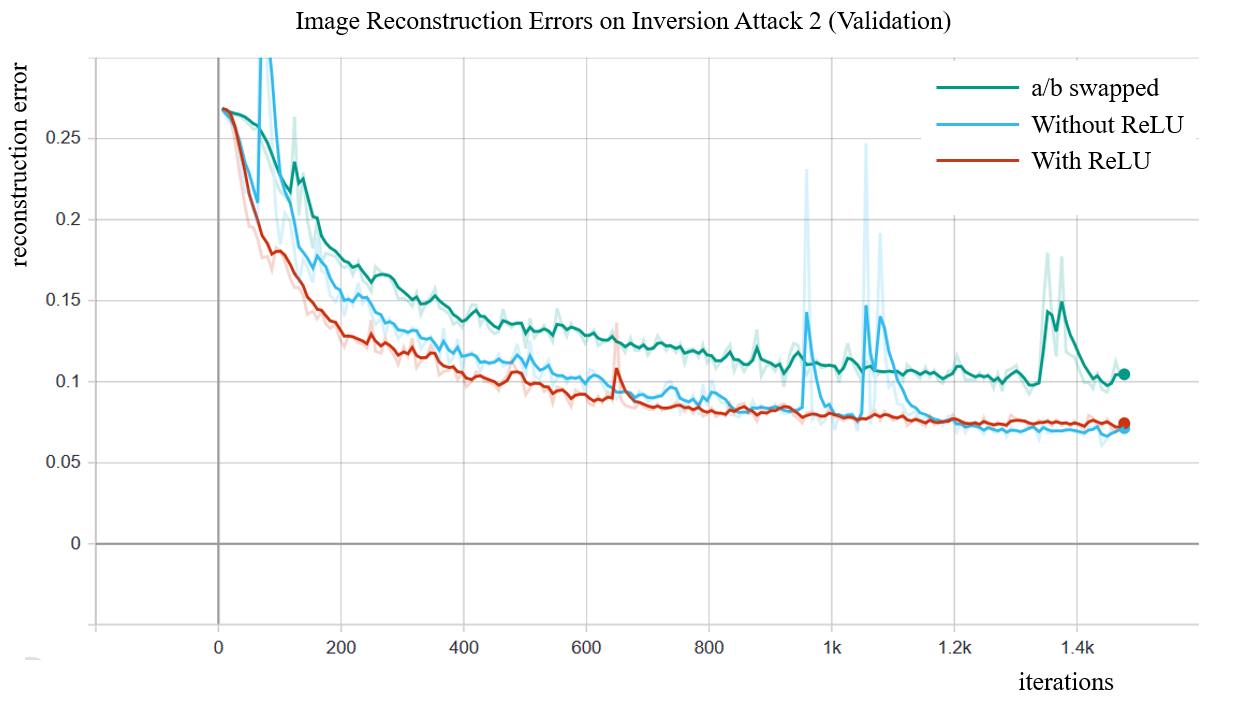
\includegraphics[width=0.6\textwidth]{../openreview/images/diagram_training.png}
    \caption{Training of the adversary model. Random swapping of a and b yields a significantly higher reconstruction error. The models with and without ReLU have similar reconstruction errors, but the model without ReLU needs much longer to train as it introduces better obfuscation.}
    \label{fig:diagram_training}
\end{figure}

% \begin{table*}[t]
%     \centering
%     \scalebox{0.75}{
%     \begin{tabular}{l|c|c}
%     \hline
%     \multicolumn{1}{c|}{} & \multicolumn{2}{|c}{Classification Error} \\
%     \hline
%     \textbf{Model} & \textbf{Paper} & \textbf{Reproduced} \\
%     \hline
%     LeNet & 17.95 & 59.62 \\
%     ResNet-32-$\alpha$ & 10.48 & 19.53 \\
%     ResNet-32-$\beta$ & 11.12 & 25.00 \\
%     ResNet-44-$\alpha$ & 11.08 & 26.09 \\
%     ResNet-44-$\beta$ & 10.51 & 26.48 \\
%     ResNet-56-$\alpha$ & 11.53 & 25.78 \\
%     ResNet-56-$\beta$ & 11.28 & 28.91 \\
%     ResNet-110-$\alpha$ & 11.97 & 24.22 \\
%     ResNet-110-$\beta$ & 11.85 & 28.17 \\
%     \end{tabular}
%     }
%     \caption{Classification Errors of the paper's results (left) and the reproduced results (right)}
%     \label{accuracy-table}
% \end{table*}

% \begin{figure}
%     \centering
%     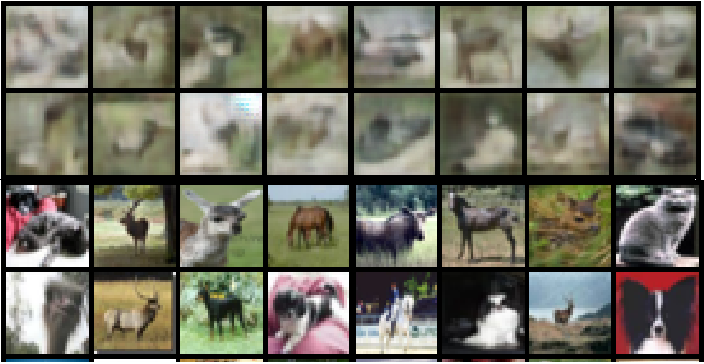
\includegraphics[width=0.3\textwidth]{../openreview/images/swap.png}
%     \caption{Image reconstructions after randomly swapping a and b. The first two rows show image reconstructions, the last two rows are the corresponding original images. The WGAN was not trained, however, the adversary is not able to reconstruct the inputs. Also, the accuracy of the classifier didn't change using this approach.}
%     \label{fig:kanonymity}
% \end{figure}

\subsection{Results beyond original paper}
% Often papers don't include enough information to fully specify their experiments, so some additional experimentation may be necessary. For example, it might be the case that batch size was not specified, and so different batch sizes need to be evaluated to reproduce the original results. Include the results of any additional experiments here. Note: this won't be necessary for all reproductions.

\subsubsection{Linear activation at the end of the generator}
The encoded features are rotated in the complex plane. Thus, their values can become negative. However, if a and b contain only positive values due to a ReLU activation at the end of the WGANs generator, finding the initial angle would be easy for an adversary. Therefore, we concluded that the ReLU has to be replaced or omitted. Empirically, we confirmed this as we found that the model spreads obfuscation and the adversary needs much more time to train. However, when training until convergence, we weren't able to confirm a significant difference in reconstruction error when compared to the model with ReLU. Reconstructed images are compared in Figure 2a-c. This underlines our general concern regarding the WGAN being too weak compared to the adversary. Again, we want to pay attention to the adversary's slow convergence rate when not using the ReLU activation. At first glance, the model seems to converge with a high reconstruction error which might lead to a wrong conclusion if training is stopped too early.

\subsubsection{K-anonymity is questionable}
There is no good way to test how the GAN is performing except training an adversary. If the adversary is trained poorly, there could be another adversary that is able to reconstruct the images much better.
To test the adversary, we disabled the training of the WGAN and instead randomly swapped the encoded features $a$ with the randomly sampled feature $b$. The decoder had access to this information and thus was able to perform as good as the normal classifier. Surprisingly, the adversary performed really poor and was not able to reconstruct the images. Instead, the adversary reconstructed an image that was very blurred and an interpolation between the two images. Our results are shown in Figure \ref{fig:kanonymity}.

Comparing the reconstructed images to the images of \cite{xiang2020interpretable}, we found that they look really similar.
This skepticism is further supported by the fact that the images shown in appendix B of \cite{xiang2020interpretable} seem to be an interpolation of two images. Finally the average angle errors shown in table 4 of \cite{xiang2020interpretable} are all $\pi/4$ except for one (VGG-16). This seems questionable since this is equal to the initial angle that lies exactly in between a and b. These reasons combined make us doubt the k-anonimity that is claimed and makes us contemplate that it is 2-anonimity instead. This 2-anonimity means that the results are just interpolations of a and b, and the attacker just has to deceiver on from the other.

All of this evidence suggests that an adversary could be able to reconstruct two images if it would be designed to do so. However, this questions the k-anonymity, which could be reduced to a 2-anonymity by selecting a better adversary.


%%%%%%%%%%%%%%%%%%%%%%%%%%%%%%%%%%%%%%%%%%%%%%%%%%%%%%%%%%%%%%%%%%%

\section{Discussion}\label{Discussion}

% Give your judgement on if your experimental results support the claims of the paper. Discuss the strengths and weaknesses of your approach - perhaps you didn't have time to run all the experiments, or perhaps you did additional experiments that further strengthened the claims in the paper.

From the results of the initial implementation of the networks (without removing the relu and adding the swapping of a and b in the generator) we can see that we do not reproduce the results of \cite{xiang2020interpretable}. Our networks don't protect the privacy as the images can be perfectly reconstructed and the properties can be perfectly inferred. Therefore the first claim (\ref{claim1}) is not supported by our results. The classification errors are however quite low and even though they are higher than those from \cite{xiang2020interpretable}, we think that with the right parameters we could have achieved the same classification errors as them. Therefore we do think that the second claim (\ref{claim2}) is supported even though our results only show partial support.

The splitting of the networks in \cite{xiang2020interpretable} is questionable. The whole idea of the paper is to have a processing unit running on the cloud so small IoT devices do not have to deal with the computational load themselves. This of course introduces privacy concerns, which the paper aims to address. However when we look at the way \cite{xiang2020interpretable} splits the networks into three parts, we see that a lot of computational effort is being put on the encoder and decoder networks. When we look at how they split the ResNet networks for example, approximately only one third of the computational effort is put on the processing unit. If this way of splitting is the only way the privacy can be protected, then it is questionable whether networks like this can actually be used on IoT devices. Also, the local device has to keep the dataset during inference in order to sample $b$. However, IoT devices lack storage capacity which could lead to major difficulties in practice.

The way \cite{xiang2020interpretable} show their results of the inference attacks is questionable as well. They decided to evaluate the classification of the network performing the attack and the evaluation of the privacy of their network on different parts of the datasets. From an evaluation point of view, we do not understand why they did this. What is worse is that it seems they chose the dataset parts in such a way that their results seem better than they actually are. For example, they evaluate the classification on the 20 major super classes of CIFAR-100, but they evaluate the privacy on all 100 classes. By definition this means that the privacy error will be higher than the classification error, which is exactly what they want, hence why it seems a bit like cheating.

The choice of the U-Net as the adversary is unclear to us. We don't see any value in first upsampling the features followed by downsampling them in the first part of the U-Net. In addition, the input of the U-Net has no important low-level features as they are upscaled, so the value of the skip connections is questionable to us. We think it'd be sufficient if the adversary consists of a simple decoder that reconstructs images by upsampling and applying convolutions.

\subsection{What was easy}
% Give your judgement of what was easy to reproduce. Perhaps the author's code is clearly written and easy to run, so it was easy to verify the majority of original claims. Or, the explanation in the paper was really easy to follow and put into code. 

% Be careful not to give sweeping generalizations. Something that is easy for you might be difficult to others. Put what was easy in context and explain why it was easy (e.g. code had extensive API documentation and a lot of examples that matched experiments in papers). 

Overall we found \cite{xiang2020interpretable} quite difficult to understand and reproduce, but what did make it a lot easier was the different implementations that were already online. For most networks that they used we found an implementation online that we could use and especially the complex neural network implementations were very useful. 

\begin{itemize}
    \item Datasets, such as CIFAR-10 (\cite{cifar10}), CIFAR-100 (\cite{cifar100}, CelebA (\cite{CelebA}) are publicly available and are easy to get access to.
    \item Main architecture for the privacy model is based on the existing and well-documented architectures such as ResNet (\cite{DBLP:journals/corr/HeZRS15}), LeNet(\cite{lecun1998gradient}), AlexNet(\cite{AlexNet}) etc.
\end{itemize}

% \begin{table*}[t]
%     \centering
%     \begin{tabular}{l||c}
%     \hline
%     \textbf{Model} & \textbf{Average Error} \\
%     \hline
%     LeNet & ? \\
%     % ResNet-20-$\alpha$ & 10.91 & ? & 0.2664 & ? & 0.2420 & ? \\
%     % ResNet-20-$\beta$ & 12.28 & ? & 0.2424 & ? & 0.2420 & ? \\
%     ResNet-32-$\alpha$ & 0.0260 \\
%     ResNet-32-$\beta$ & 0.0265 \\
%     % ResNet-44-$\alpha$ & 11.08 & ? & 0.2746 & ? & 0.2419 & ? \\
%     % ResNet-44-$\beta$ & 10.51 & ? & 0.2511 & ? & 0.2397 & ? \\
%     ResNet-56-$\alpha$ & ? \\
%     ResNet-56-$\beta$ & ? \\
%     ResNet-110-$\alpha$ & 0.0320 \\
%     ResNet-110-$\beta$ & 0.0403 \\
%     \end{tabular}
%     \caption{Average error of predicting the angle}
%     \label{angle-table}
% \end{table*}

\subsection{What was difficult}
% List part of the reproduction study that took more time than you anticipated or you felt were difficult. 

Some crucial details such as discriminator architecture and major hyper-parameters were not included in the publication, making it difficult to properly replicate the results with sufficient precision. One of the main hyper-parameters that were missing were the learning rates, optimizers and weight decay values that were used. This particularly, made implementation of WGAN vague and we had to make a lot of assumptions. This is especially a problem, since the WGAN is the only part that can provide the privacy protection, so if the WGAN does not work properly we cannot achieve the privacy protection that they claim in the paper.

Description of the inversion attacks (1) and (2) mentioned in section 4.3 were not consistent with the description of experiments in section 5. For example, the authors state in the section 4.3 of the paper that inversion attack 1 implies  estimation of proper angle $\hat{\theta}$, which would allow the estimation of original features $a*$, which could be later passed to inversion model. Additionally, the description also implies the discriminator that is used to train the angle-prediction. In the implementation part of section 5, authors state that the inversion model is based on the U-Net, however, there was no architecture description of the angle-estimator (which we assumed is an another neural network), nor discriminator that is used for training of such estimator. What obfuscates it further is the fact that the authors did not make clear distinctions between the aforementioned attacks (1) and (2) in the "implementation details" section, confusing as to which attack and in what way does the aforementioned U-Net architecture actually relate.

% Authors left very little information about loss measures, leaving only information about evaluation metrics. Because of that, relevant metrics for attack were not available to us.

% Be careful to put your discussion in context. For example, don't say "the maths was difficult to follow", say "the math requires advanced knowledge of calculus to follow". 

% \subsection{Communication with original authors}
% Document the extent of (or lack of) communication with the original authors. To make sure the reproducibility report is a fair assessment of the original research, we recommend getting in touch with the original authors. You can ask authors specific questions, or if you don't have any questions, you can send them the full report to get their feedback before it gets published. 
% We did not contact the original authors of the publication. 
%%%%%%%%%%%%%%%%%%%%%%%%%%%%%%%%%%%%%%%%%%%%%%%%%%%%%%%%%%%%%%%%%%%

% \section*{References}
\newpage
\bibliography{refs}
\bibliographystyle{neurips_natbib}